\chapter{Aplicația Dezvoltată}
\label{chap:application}

% ----------------------------------------------------------------
\section{Specificarea aplicației}
\label{sec:specs}

Aplicația este un sistem full-stack pentru analiza și predicția
probabilității de câștig în meciuri de fotbal din Liga 1 a României
(Superliga), care integrează modelul LightGBM antrenat pe date StatsBomb
(Capitolul~\ref{cap:metodologie}) cu date despre meciuri reale provenite
din serviciul comercial API-Football. API-Football este o interfață de
programare (REST API) care expune date sportive structurate (clasamente,
meciuri, statistici și evenimente de joc) pentru un număr mare de
competiții; în cadrul acestei lucrări este folosit ca sursă de date pentru
Superligă. Datele sunt accesate prin planul gratuit al API-Football, care
limitează accesul la sezonul 2023, astfel încât aplicația operează exclusiv
pe meciurile din sezonul 2023 al Superligii (identificator de ligă 283).

Sistemul permite unui utilizator autentificat să consulte clasamentul și
meciurile finalizate ale sezonului, să genereze o predicție probabilistică
pentru un meci selectat și să își regăsească predicțiile salvate, organizate
pe echipe. Figura~\ref{fig:usecase} prezintă diagrama Use Case a aplicației,
care sintetizează interacțiunile dintre utilizator și principalele
funcționalități ale sistemului.

\begin{figure}[H]
    \centering
    
\includegraphics[width=0.85\textwidth]{figures/usecase_diagram.png}
    \caption{Diagrama Use Case a aplicației, ilustrând acțiunile pe care le
    poate efectua un utilizator autentificat.}
    \label{fig:usecase}
\end{figure}

\subsection{Cerințe funcționale}

Cerințele funcționale descriu comportamentul observabil al sistemului din
perspectiva utilizatorului. Aplicația trebuie să asigure următoarele
funcționalități:

\begin{itemize}
    \item \textbf{Autentificarea utilizatorilor} prin înregistrare și
    autentificare cu token JWT, astfel încât fiecare utilizator să aibă un
    spațiu de date propriu și protejat.
    \item \textbf{Vizualizarea clasamentului} actualizat al Superligii
    pentru sezonul 2023, pentru a oferi utilizatorului contextul competitiv
    al echipelor.
    \item \textbf{Vizualizarea meciurilor finalizate} din sezon, listă din
    care utilizatorul selectează meciul pentru care dorește o analiză.
    \item \textbf{Generarea unei predicții} pentru un meci finalizat
    selectat, pe baza datelor extrase automat din API-Football, fără ca
    utilizatorul să introducă manual statistici.
    \item \textbf{Afișarea probabilităților} de victorie gazdă, egal și
    victorie oaspeți, împreună cu evoluția lor pe parcursul meciului și cu
    momentele decisive identificate.
    \item \textbf{Salvarea predicției} în istoricul utilizatorului, pentru a
    permite consultarea ulterioară.
    \item \textbf{Vizualizarea predicțiilor salvate}, organizate pe echipe,
    pentru a urmări evoluția probabilistică a unei echipe de-a lungul
    sezonului.
\end{itemize}

\subsection{Cerințe non-funcționale}

Cerințele non-funcționale descriu constrângerile de calitate ale
sistemului. Timpul de răspuns pentru generarea unei predicții trebuie să
rămână sub 2 secunde, în condițiile în care procesul include și apelurile
către API-Football. Din punct de vedere al securității, parolele sunt
stocate folosind funcția de hashing bcrypt, accesul este controlat prin
tokeni JWT cu expirare la 24 de ore, iar datele de intrare sunt validate
strict cu ajutorul schemelor Pydantic. Pentru a reduce numărul de apeluri
către API-Football (limitat de planul gratuit), backend-ul folosește un
cache în memorie pentru clasament și meciuri, cu un interval de valabilitate
configurabil. Comunicarea între frontend și backend este permisă prin
configurarea CORS pentru originile de dezvoltare, iar interfața este
proiectată să fie responsivă, funcționând atât pe dispozitive desktop, cât
și mobile.

% ----------------------------------------------------------------
\section{Proiectarea sistemului}
\label{sec:design}

\subsection{Arhitectura sistemului}

Sistemul urmează o arhitectură three-tier (pe trei niveluri): un nivel de
prezentare (frontend React), un nivel de logică de aplicație (backend
FastAPI) și un nivel de date (sistemul de fișiere local și sursele externe
de date). Frontend-ul comunică prin HTTP/REST cu backend-ul, care la rândul
său orchestrează inferența modelului de învățare automată, apelurile către
API-Football și persistența datelor. Figura~\ref{fig:arhitectura} prezintă
această organizare pe niveluri.

\begin{figure}[H]
    \centering
    
\includegraphics[width=0.88\textwidth]{figures/arhitectura_sistem.png}
    \caption{Arhitectura three-tier a aplicației, cu separarea dintre
    nivelul de prezentare, nivelul de logică și nivelul de date.}
    \label{fig:arhitectura}
\end{figure}

Persistența datelor este asigurată prin stocare directă în fișiere JSON pe
server, organizate în directoare separate pentru utilizatori
(\texttt{/users/}) și pentru predicții (\texttt{/predictions/}), fără a
necesita un sistem de baze de date dedicat. Aceasta este o abordare
deliberat simplificată, adecvată volumului redus de date și scopului
academic al lucrării. Trebuie remarcat că, în această variantă, datele sunt
stocate necriptat pe disc, iar izolarea între utilizatori este asigurată la
nivel de aplicație (prin verificarea identității din token-ul JWT înainte de
accesarea fișierului corespunzător); o variantă de producție ar necesita o
bază de date cu control de acces și criptare la nivel de stocare, aspect
discutat în capitolul de concluzii.

\subsection{Fluxul de date pentru generarea unei predicții}

Fluxul principal de date pentru generarea unei predicții, ilustrat în
Figura~\ref{fig:sequence}, începe în momentul în care frontend-ul trimite
identificatorul meciului (\texttt{fixture\_id}) către endpoint-ul
\texttt{POST /predict/by-fixture-id}. Backend-ul apelează în secvență
endpoint-urile \texttt{/fixtures/statistics} și \texttt{/fixtures/events}
din API-Football, mapează răspunsul la structura internă \texttt{MatchInput}
prin modulul \texttt{api\_football\_mapper.py}, rulează inferența modelului
LightGBM și returnează probabilitățile către frontend. Predicția rezultată
este salvată imediat în fișierul \texttt{/predictions/\{user\_id\}.json}.

\begin{figure}[H]
    \centering
    
\includegraphics[width=0.88\textwidth]{figures/sequence_diagram.png}
    \caption{Diagrama de secvență pentru generarea unei predicții, de la
    cererea frontend-ului până la salvarea rezultatului.}
    \label{fig:sequence}
\end{figure}

\subsection{Componentele backend-ului}

Backend-ul este structurat modular, fiecare fișier având o
responsabilitate bine delimitată, conform principiului separării
responsabilităților. Tabelul~\ref{TabelBackend} prezintă rolul fiecărui
modul. Punctul de intrare (\texttt{app.py}) definește rutele și
middleware-ul, schemele de date (\texttt{models.py}) impun structura
cererilor și răspunsurilor, autentificarea (\texttt{auth.py}) și gestionarea
utilizatorilor (\texttt{users.py}) tratează identitatea, iar inferența
modelului (\texttt{predictions.py}) și maparea datelor externe
(\texttt{api\_football\_mapper.py}) implementează logica de predicție.
Această separare permite modificarea unei componente (de exemplu
înlocuirea modelului) fără a afecta restul sistemului.

\begin{table}[htbp]
\begin{center}
\begin{tabular}{|p{130pt}|p{230pt}|}
\hline
\textbf{Fișier} & \textbf{Rol} \\
\hline
\texttt{app.py} & Rute FastAPI, configurare CORS, middleware de logging \\
\hline
\texttt{models.py} & Scheme Pydantic: MatchInput, PredictionResponse \\
\hline
\texttt{auth.py} & Generare și validare tokeni JWT \\
\hline
\texttt{predictions.py} & Încărcarea modelului și inferența \\
\hline
\texttt{api\_football\_mapper.py} & Conversia răspunsului API-Football în
MatchInput \\
\hline
\texttt{config.py} & Variabile de mediu și chei API \\
\hline
\texttt{users.py} & Gestionarea utilizatorilor: creare, autentificare,
stocare JSON \\
\hline
\end{tabular}
\end{center}
\caption{Componentele backend-ului și rolul fiecăruia.}
\label{TabelBackend}
\end{table}

% ----------------------------------------------------------------
\section{Tehnologii utilizate}
\label{sec:tehnologii}

Nivelul de prezentare este construit cu \textbf{React}, o bibliotecă
JavaScript pentru construirea interfețelor utilizator bazată pe o
arhitectură orientată pe componente, în care fiecare componentă încapsulează
atât logica, cât și reprezentarea vizuală (JSX), iar interfețele complexe
sunt construite prin compunerea componentelor simple. Pentru managementul
stării globale (în special starea de autentificare) este folosit
\textbf{Context API}, mecanismul nativ React care evită problema
\textit{prop drilling}, adică transmiterea datelor prin lanțuri lungi de
componente intermediare. Aplicația este servită și împachetată cu
\textbf{Vite}, un instrument de build modern care utilizează module ES
native în browser în timpul dezvoltării, reducând semnificativ timpul de
pornire a serverului de dezvoltare față de soluțiile clasice. Pentru
graficele interactive este folosită biblioteca \textbf{Recharts}, iar pentru
navigarea între pagini biblioteca \textbf{React Router}.

Nivelul de logică este implementat în Python cu \textbf{FastAPI}, un cadru
web modern pentru construirea de API-uri REST, ales pentru performanța sa,
pentru validarea automată a datelor prin Pydantic și pentru documentația
interactivă generată automat (Swagger UI).

Integrarea cu API-Football urmează modelul arhitectural
\textit{Backend for Frontend} (BFF): în loc ca frontend-ul să apeleze direct
serviciul extern, toate cererile sunt rutate prin propriul backend, care
agregă, transformă și păstrează temporar (cache) datele înainte de a le
returna clientului. Avantajele acestei abordări sunt triple: cheia API
rămâne secretă pe server, răspunsurile pot fi cache-uite centralizat, iar
formatul datelor poate fi adaptat nevoilor frontend-ului independent de
structura API-ului extern. Cache-ul în memorie cu interval de valabilitate
(TTL, Time To Live) stochează temporar rezultatul unui apel costisitor și îl
reutilizează pentru cererile ulterioare până la expirarea intervalului
configurat, reducând atât latența percepută, cât și numărul de apeluri
consumate din cota planului gratuit.

% ----------------------------------------------------------------
\section{Implementare}
\label{sec:implementation}

\subsection{Backend (FastAPI)}

Backend-ul expune endpoint-urile necesare pentru autentificare, accesul la
datele Superligii și generarea predicțiilor. Comunicarea cu API-Football
este realizată prin apeluri HTTP directe (biblioteca \texttt{urllib}), fără
biblioteci externe suplimentare. Endpoint-urile principale sunt:

\begin{itemize}
    \item \texttt{POST /auth/register} pentru crearea unui cont nou;
    credențialele sunt stocate în \texttt{/users/\{user\_id\}.json}, parola
    fiind hash-uită cu bcrypt;
    \item \texttt{POST /auth/login} pentru autentificare și returnarea unui
    token JWT cu expirare de 24 de ore;
    \item \texttt{GET /users/me} pentru profilul utilizatorului autentificat;
    \item \texttt{GET /api/superliga/standings} pentru clasamentul
    Superligii, rutat din API-Football cu cache în memorie;
    \item \texttt{GET /api/superliga/fixtures/\{season\}} pentru lista
    meciurilor din sezonul selectat, cu indicarea, pentru fiecare meci, dacă
    utilizatorul curent a generat deja o predicție;
    \item \texttt{POST /predict/by-fixture-id} pentru generarea unei
    predicții pe baza unui \texttt{fixture\_id}, backend-ul preluând automat
    statisticile și evenimentele din API-Football;
    \item \texttt{GET /matches} pentru toate predicțiile salvate ale
    utilizatorului;
    \item \texttt{GET /health} pentru starea serverului și a modelului
    încărcat.
\end{itemize}

Pentru a limita numărul de apeluri către API-Football, backend-ul
implementează un cache în memorie pentru clasament și meciuri, cu un interval
de valabilitate configurabil prin variabila \texttt{SUPERLIGA\_CACHE\_SECONDS}
din \texttt{config.py}. La fiecare cerere se verifică dacă datele din cache
sunt încă valide; în caz contrar, se efectuează un nou apel către API și se
actualizează cache-ul.

Maparea datelor externe este realizată de modulul
\texttt{api\_football\_mapper.py}, care convertește răspunsul API-Football la
structura \texttt{MatchInput} așteptată de model. Procesul extrage din
statistici șuturile totale și pe poartă, pasele, posesia procentuală și
expected goals (xG). Cartonașele sunt numărate din lista de evenimente, nu
din statisticile agregate, pentru a asigura acuratețea per echipă, iar
posesia procentuală este mapată pe câmpul \texttt{pressure} din
\texttt{MatchInput}, ca aproximare a presiunii exercitate. Persistența
datelor se realizează prin fișiere JSON pe server, câte un fișier per
utilizator, ceea ce elimină dependența de un sistem de baze de date extern
și simplifică deployment-ul. Figura~\ref{fig:backend_flow} ilustrează fluxul
intern de procesare pentru endpoint-ul de predicție.

\begin{figure}[H]
    \centering
    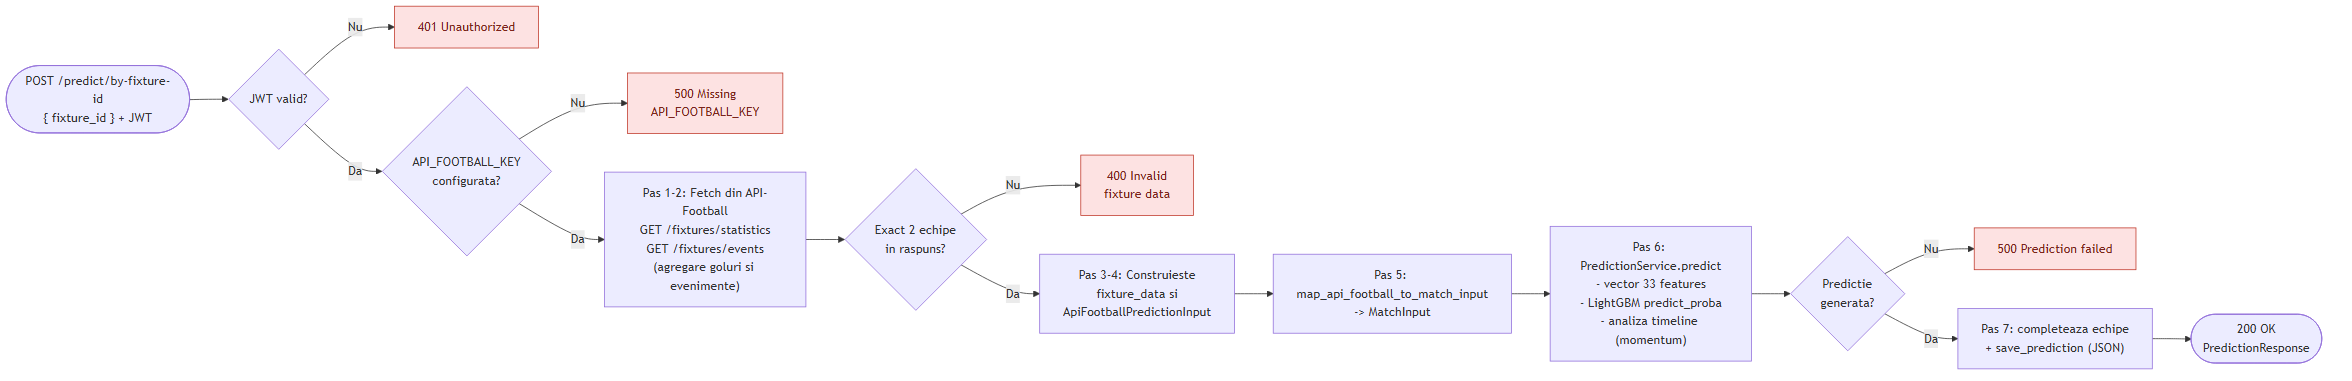
\includegraphics[width=0.9\textwidth]{figures/backend_flow.png}
    \caption{Fluxul intern de procesare pentru
    \texttt{POST /predict/by-fixture-id}, de la primirea cererii până la
    returnarea probabilităților.}
    \label{fig:backend_flow}
\end{figure}

\subsection{Frontend (React)}

Interfața este organizată conform unei separări clare pe niveluri:
componente de prezentare, un strat de servicii pentru comunicarea cu
backend-ul, un context global pentru autentificare și hook-uri
personalizate pentru reutilizarea logicii. Aplicația este structurată în
cinci pagini principale (autentificare, prezentare, clasament, meciuri și
analiza unui meci), gestionate prin React Router.

Controlul accesului este implementat prin două componente de rutare
declarativă: o componentă \texttt{ProtectedRoute}, care redirecționează
către pagina de autentificare utilizatorii neautentificați, și o componentă
\texttt{PublicRoute}, care redirecționează utilizatorii deja autentificați
către pagina principală. Starea de autentificare (token-ul JWT și datele
utilizatorului) este gestionată central printr-un \texttt{AuthContext}, expus
componentelor prin hook-ul personalizat \texttt{useAuth}. La pornirea
aplicației, contextul încearcă să restabilească sesiunea pe baza token-ului
din \texttt{localStorage}, validându-l printr-un apel la \texttt{GET /users/me}.

Comunicarea cu backend-ul este izolată într-un strat de servicii organizat
ca obiecte singleton: un serviciu HTTP generic (\texttt{ApiService}),
construit peste API-ul nativ \texttt{fetch} al browserului, și servicii
specializate pentru autentificare, pentru datele Superligii și pentru
predicții. Serviciul HTTP generic centralizează construirea adreselor,
serializarea JSON, tratarea uniformă a erorilor și un mecanism de timeout
implementat cu \texttt{AbortController}; token-ul de autentificare este
atașat automat ca antet \texttt{Authorization} pe acest serviciu după
autentificare. Pentru a reduce traficul, serviciul Superligii implementează
un cache în \texttt{localStorage} cu versionare și interval de valabilitate
(șase ore) pentru lista de meciuri, cu revenire la cache-ul expirat atunci
când rețeaua este indisponibilă.

Pagina de analiză a unui meci agregă patru componente vizuale, construite pe
baza răspunsului de la backend și a unor prelucrări suplimentare efectuate
pe partea de client în serviciul de predicții. Componenta
\texttt{WinProbabilityChart}, realizată cu Recharts, reprezintă grafic
evoluția probabilităților de-a lungul meciului. Componenta
\texttt{ProbabilityCard} afișează predicția finală sub forma a trei carduri,
cu probabilitatea fiecărui rezultat și un indicator de încredere. Componenta
\texttt{KeyEvents} listează cronologic momentele decisive, iar componenta
\texttt{MatchInsights} sintetizează automat statistici cheie ale meciului.
O parte din aceste statistici sunt derivate pe partea de client: împărțirea
meciului pe intervale de dominanță (funcția \texttt{deriveDominancePeriods}),
identificarea perioadei celei mai volatile (\texttt{deriveMostVolatilePeriod})
și a evenimentului cu cel mai mare impact (\texttt{deriveBiggestSwing}),
precum și distribuția golurilor pe echipe (\texttt{deriveGoalsBreakdown}).
Aspectul efectiv al acestor componente, din perspectiva utilizatorului, este
prezentat în Secțiunea~\ref{sec:userguide}.

% ----------------------------------------------------------------
\section{Testare}
\label{sec:testing}

Testarea aplicației a acoperit trei niveluri: testarea endpoint-urilor
backend, testarea integrării cu API-Football și testarea interfeței
frontend.

Testarea backend a combinat verificarea manuală prin Swagger UI
(\texttt{/docs}) cu un script automat de tip smoke-test,
\texttt{tests/test\_api.py}, care parcurge secvențial principalele
endpoint-uri (\texttt{/health}, \texttt{/auth/register}, \texttt{/auth/login},
\texttt{/users/me}, \texttt{/predict} și \texttt{/matches}) și confirmă că
fluxul complet funcționează de la un capăt la altul. Prin Swagger UI au fost
verificate răspunsurile pentru scenarii valide și invalide: token expirat sau
lipsă (cod 401), utilizator inexistent (404), \texttt{fixture\_id} invalid
(400) și depășirea limitei de apeluri API-Football (429). Endpoint-ul
\texttt{POST /predict/by-fixture-id} a fost validat pe 10 meciuri reale din
Superliga 2023, comparând probabilitățile generate cu rezultatele cunoscute.
Trebuie precizat că această testare este una funcțională, bazată pe script și
pe verificare manuală, și nu o suită de teste unitare automate cu aserțiuni;
extinderea către o astfel de suită este menționată în capitolul de concluzii
ca direcție viitoare.

Testarea integrării a urmărit fluxul complet, de la autentificare la
selectarea meciului, generarea predicției, salvarea și vizualizarea acesteia
în pagina de predicții, pentru trei utilizatori diferiți, confirmând
izolarea corectă a datelor per utilizator în sistemul de fișiere JSON. A
fost verificată și funcționarea cache-ului: un al doilea apel către
\texttt{/api/superliga/standings} în intervalul de valabilitate returnează
datele din memorie fără un apel suplimentar către API-Football.

Testarea modulului de mapare \texttt{api\_football\_mapper.py} a fost
realizată pe răspunsuri reale din API-Football, verificând extragerea
corectă a statisticilor (șuturi, xG, pase, posesie) și numărarea
cartonașelor din lista de evenimente. Au fost tratate cazurile limită:
valori lipsă (\texttt{null}), procente exprimate ca șir de caractere
(de exemplu \texttt{"58\%"}) și valori de tip dicționar cu cheie
\texttt{total}. În final, interfața frontend a fost testată în Chrome și
Firefox, pe rezoluții desktop și mobile, verificând comportamentul responsiv
și afișarea corectă a datelor returnate de backend.

% ----------------------------------------------------------------
\section{Manualul utilizatorului}
\label{sec:userguide}

Această secțiune descrie utilizarea aplicației din perspectiva
utilizatorului final, pas cu pas.

\textbf{Pasul 1, autentificarea.} La accesarea aplicației, utilizatorul este
direcționat către pagina de autentificare (Figura~\ref{fig:manual_login}).
Un cont nou poate fi creat prin butonul \textit{Register}, completând
email-ul, parola și numele complet. După autentificare, sesiunea rămâne
activă 24 de ore.

\begin{figure}[H]
    \centering
    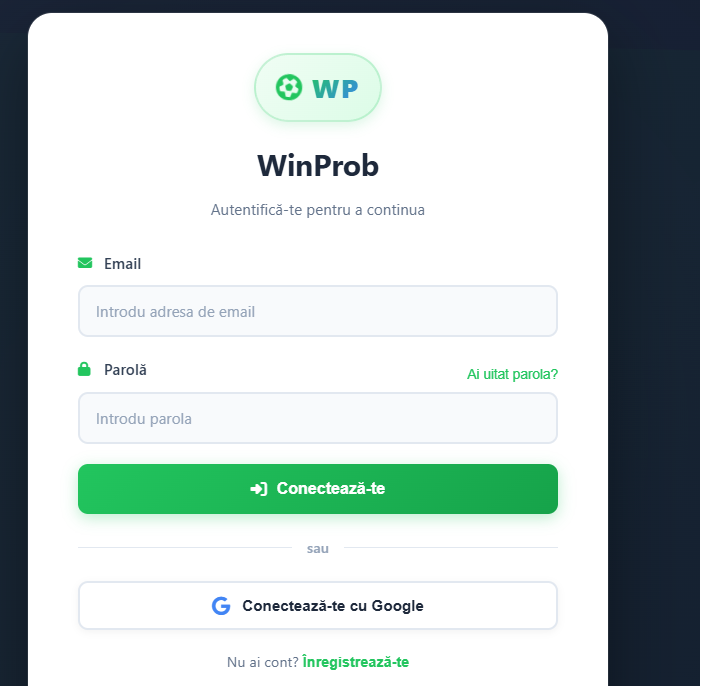
\includegraphics[width=0.82\textwidth]{figures/screenshot_login.png}
    \caption{Pagina de autentificare și înregistrare.}
    \label{fig:manual_login}
\end{figure}

\textbf{Pasul 2, navigarea.} După autentificare, meniul de navigare oferă
acces la toate secțiunile aplicației: pagina de prezentare (\textit{Acasă}),
\textit{Clasament}, \textit{Meciuri} și \textit{Predicții}. Pagina de
prezentare introduce utilizatorul în contextul aplicației, descriind scopul
și funcționalitățile disponibile.

\textbf{Pasul 3, vizualizarea clasamentului.} Din pagina \textit{Clasament}
(Figura~\ref{fig:standings}), utilizatorul vede situația actuală a tuturor
echipelor din Superliga, sezonul 2023. Pentru fiecare echipă sunt afișate
poziția, numărul de meciuri jucate, victoriile, egalurile, înfrângerile,
golurile marcate și primite, golaverajul și punctele.

\begin{figure}[H]
    \centering
    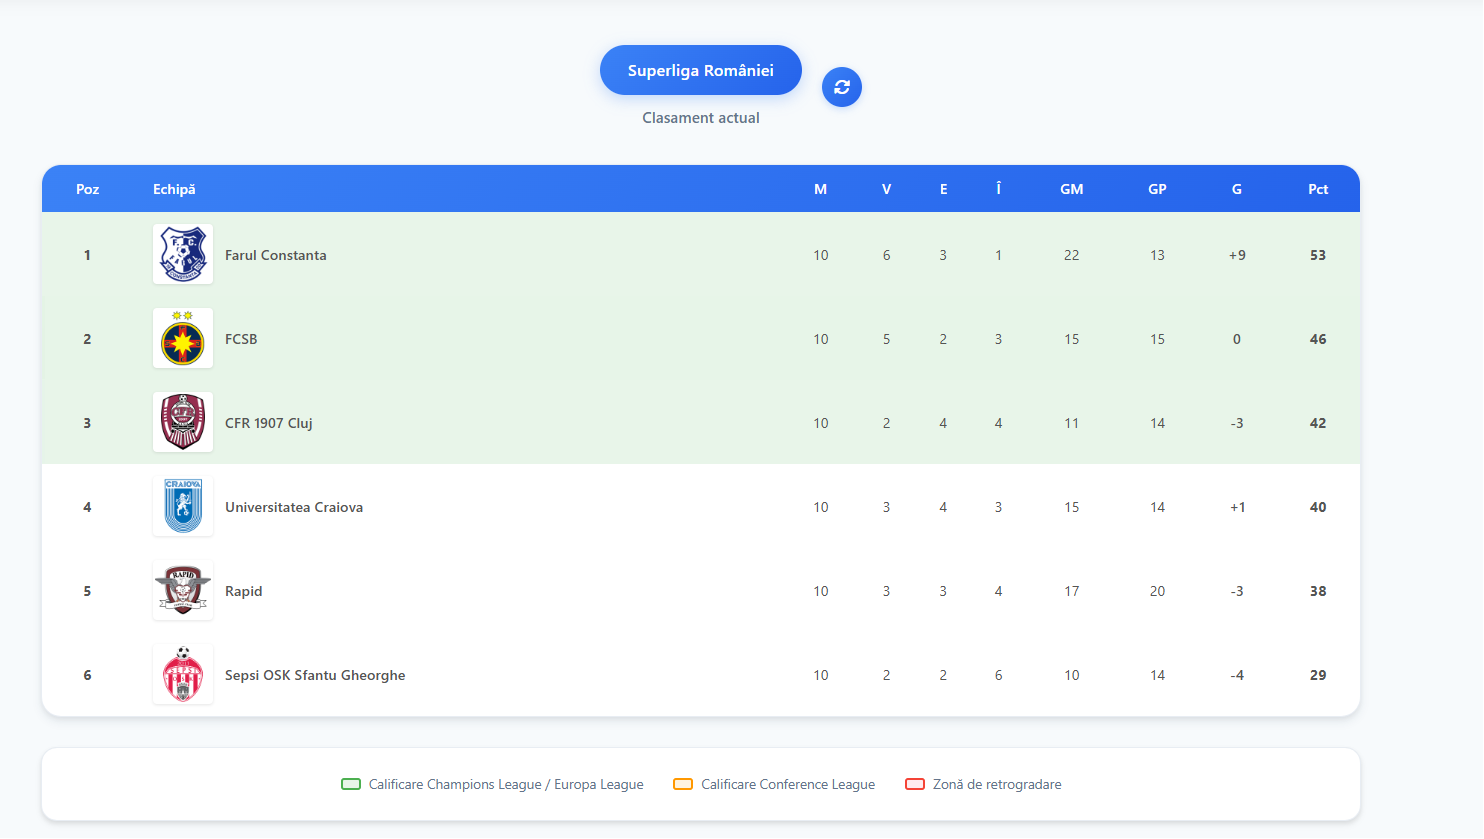
\includegraphics[width=0.85\textwidth]{figures/screenshot_standings.png}
    \caption{Pagina de clasament a Superligii.}
    \label{fig:standings}
\end{figure}

\textbf{Pasul 4, generarea unei predicții.} Din pagina \textit{Meciuri}
(Figura~\ref{fig:matches}), utilizatorul selectează un meci finalizat din
lista disponibilă. Pe pagina de detalii a meciului apasă butonul
\textit{Generează predicție}. Backend-ul preia automat statisticile și
evenimentele meciului din API-Football, le procesează prin mapper și rulează
inferența pe modelul LightGBM, iar rezultatul este afișat
(Figura~\ref{fig:result}).

\begin{figure}[H]
    \centering
    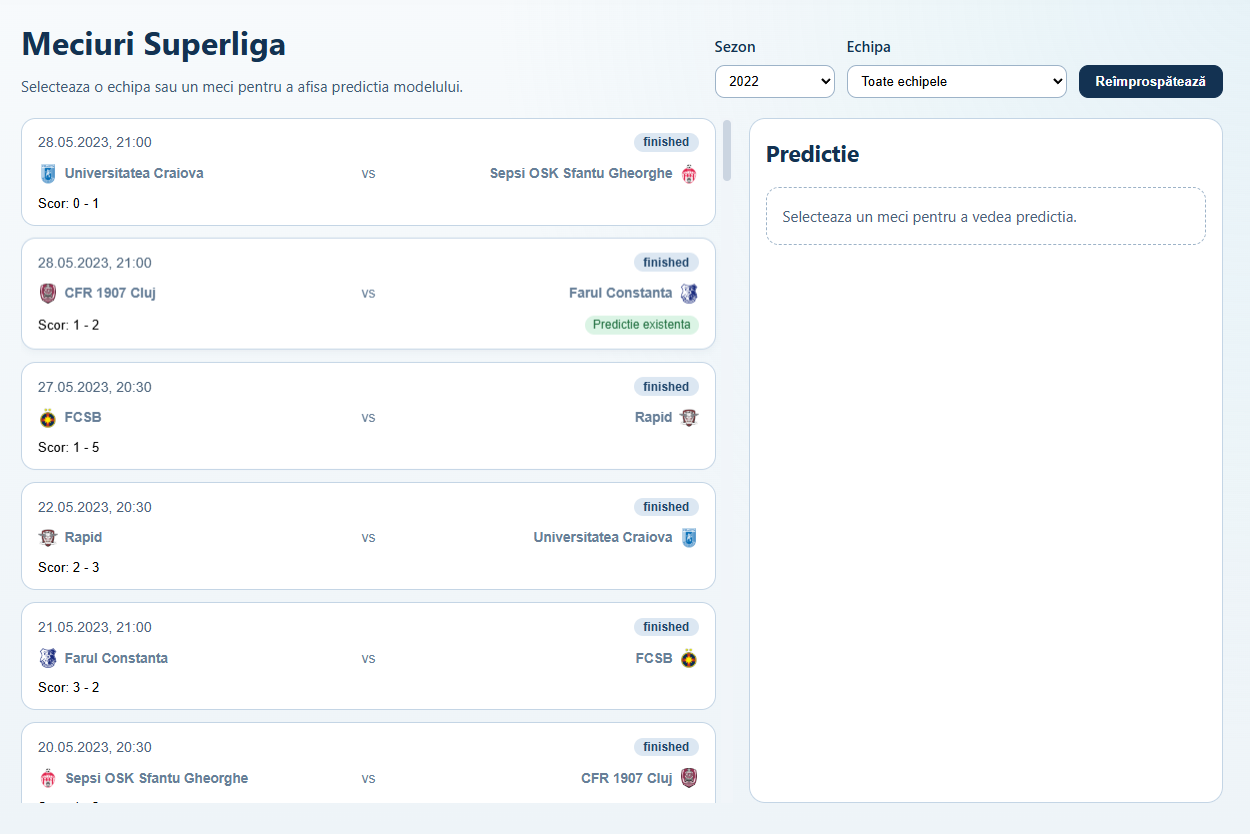
\includegraphics[width=0.85\textwidth]{figures/screenshot_matches.png}
    \caption{Lista meciurilor finalizate și detaliile unui meci selectat.}
    \label{fig:matches}
\end{figure}

\begin{figure}[H]
    \centering
    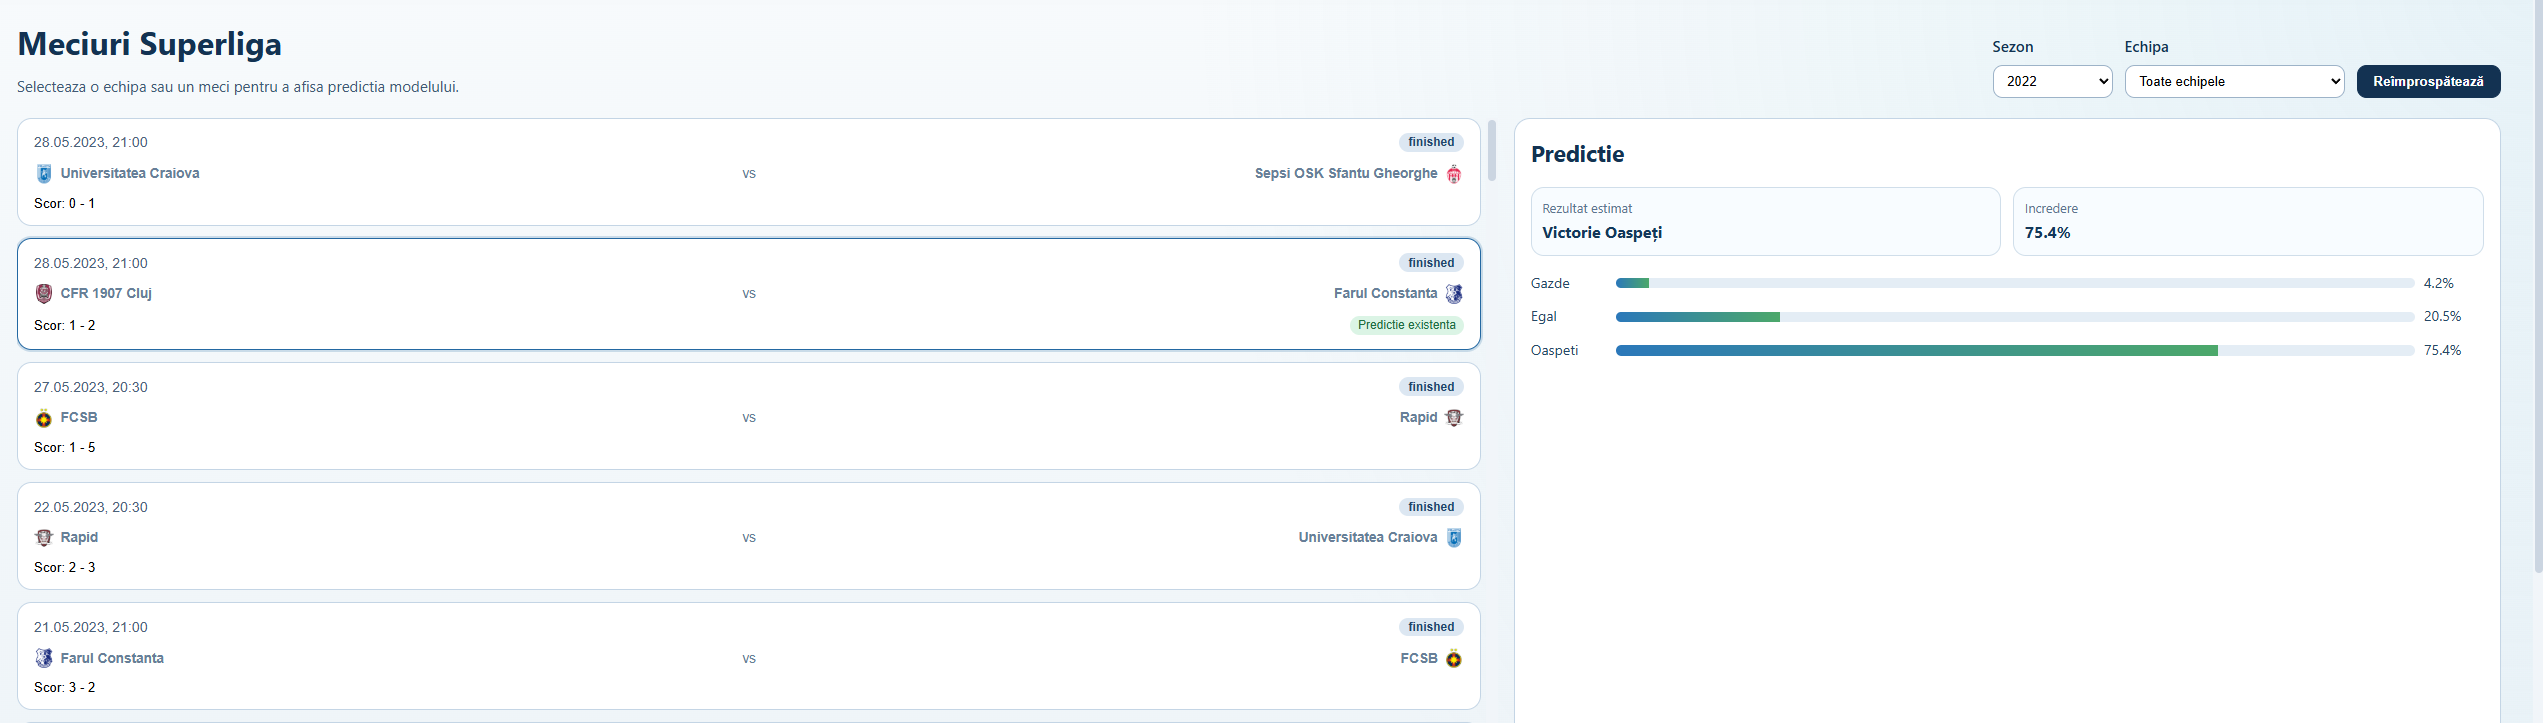
\includegraphics[width=0.85\textwidth]{figures/screenshot_result.png}
    \caption{Rezultatul unei predicții: probabilitățile de victorie gazdă,
    egal și victorie oaspeți.}
    \label{fig:result}
\end{figure}

Pagina de analiză a unui meci conține patru componente. Prima este graficul
evoluției probabilității de victorie (Figura~\ref{fig:prob_chart}), care
reconstituie dinamica meciului eveniment cu eveniment: axa orizontală
reprezintă minutele în care au avut loc evenimente relevante, iar axa
verticală indică probabilitatea curentă pentru fiecare rezultat, momentele
decisive (în special golurile) fiind marcate explicit pe grafic.

\begin{figure}[H]
    \centering
    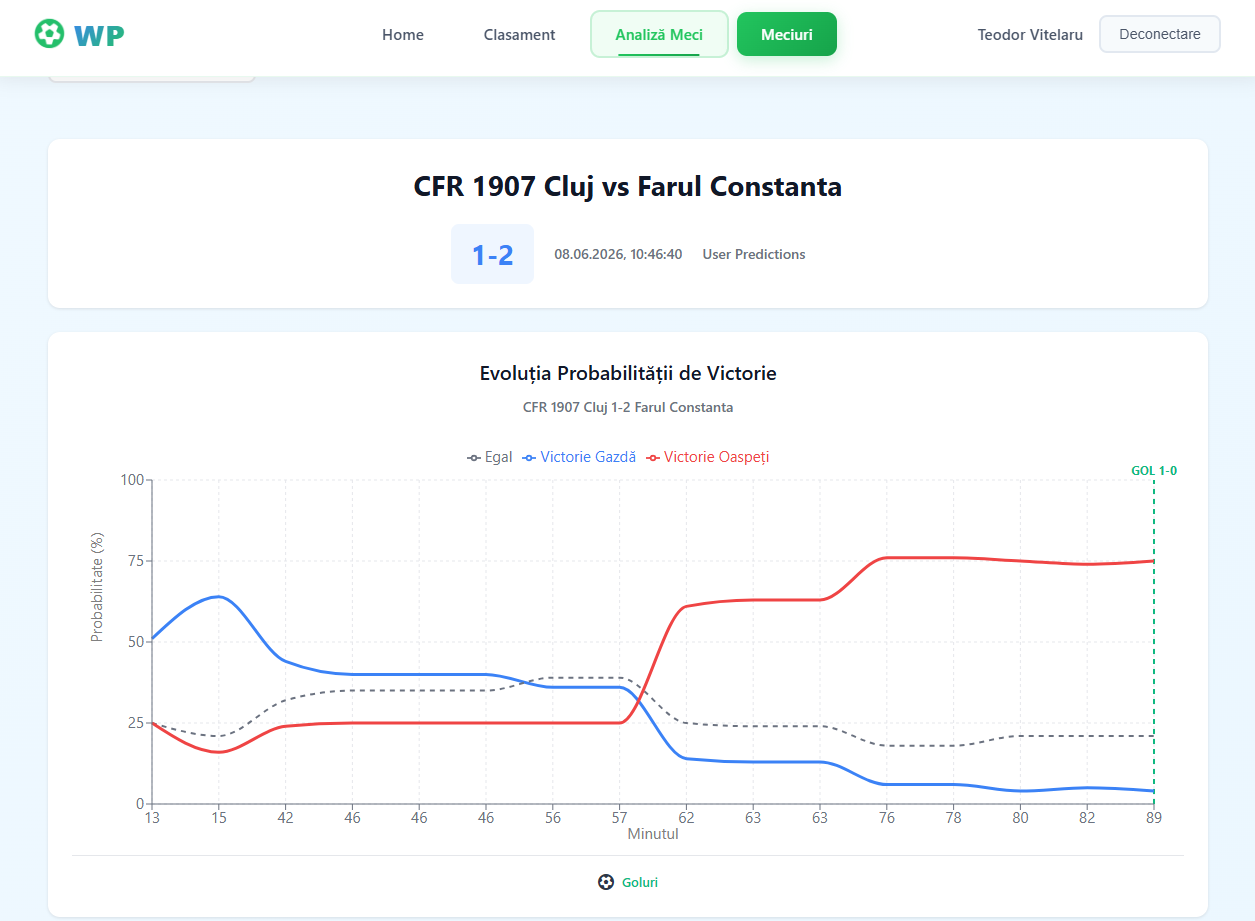
\includegraphics[width=0.85\textwidth]{figures/descriere1.png}
    \caption{Evoluția probabilității de victorie de-a lungul meciului
    CFR 1907 Cluj contra Farul Constanța (1-2). Graficul ilustrează
    inversarea echipei favorite: CFR Cluj pornește cu o probabilitate de
    câștig de circa 50\%, care crește la 63\% după golul din minutul 15,
    pentru ca în minutul 62 Farul Constanța să preia controlul cu 60\%,
    ajungând la 75\% până la finalul partidei.}
    \label{fig:prob_chart}
\end{figure}

A doua componentă afișează predicția finală sub forma a trei carduri
(\textit{Victorie Oaspeți}, \textit{Egal} și \textit{Victorie Gazdă}), cu
probabilitatea corespunzătoare și un indicator de încredere; favorita este
evidențiată vizual. Sub predicția finală, secțiunea \textit{Key Events}
listează cronologic momentele decisive ale meciului, cu detalii despre
variația de probabilitate produsă de fiecare eveniment și jucătorul implicat
(Figura~\ref{fig:final_prediction}).

\begin{figure}[H]
    \centering
    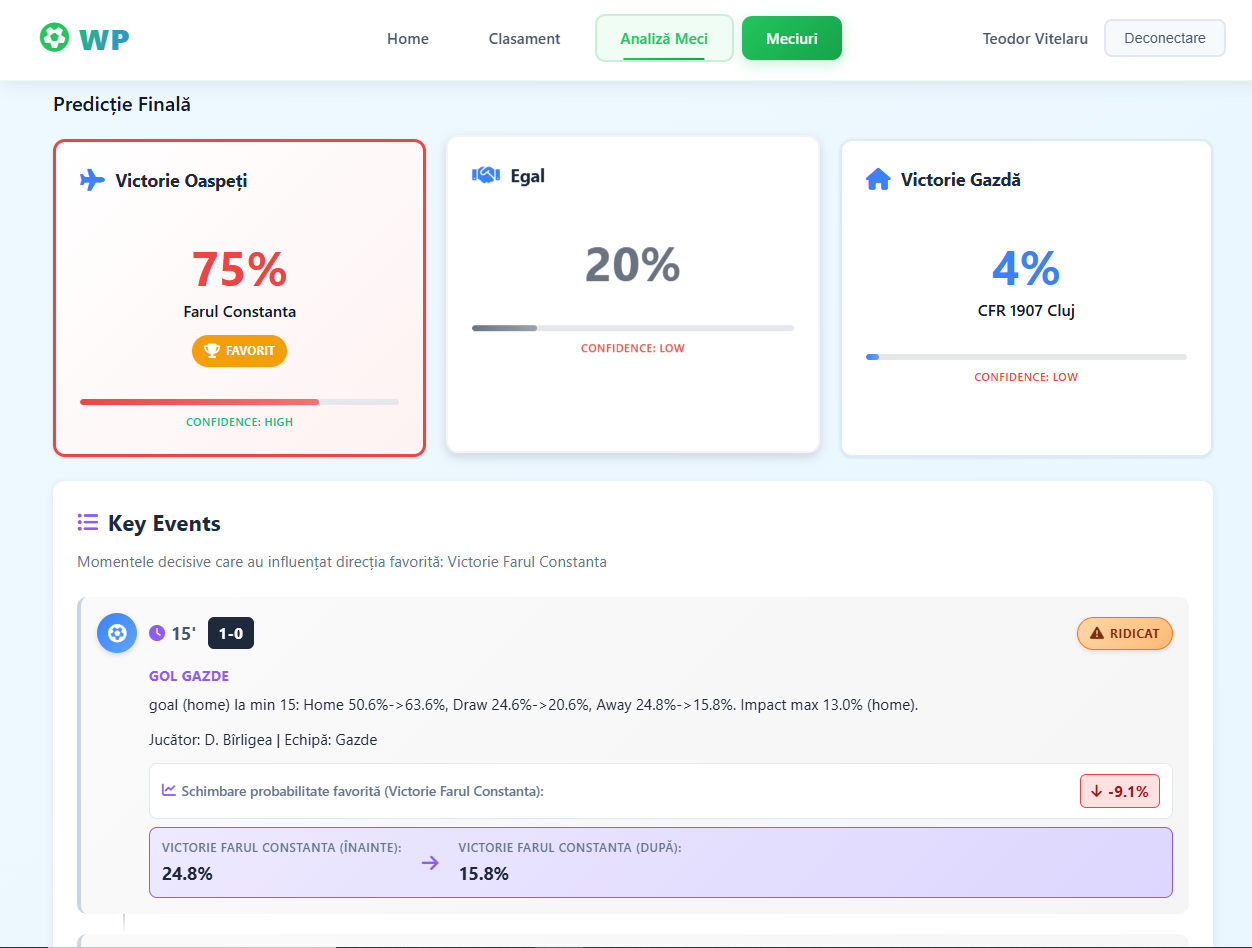
\includegraphics[width=0.85\textwidth]{figures/descriere2.png}
    \caption{Predicția finală pentru meciul CFR 1907 Cluj contra Farul
    Constanța: Victorie Oaspeți 75\%, Egal 20\%, Victorie Gazdă 4\%.
    Secțiunea \textit{Key Events} detaliază impactul golului din minutul 15
    asupra probabilităților: victoria gazdei de la 50.6\% la 63.6\%, victoria
    oaspeților de la 24.8\% la 15.8\%.}
    \label{fig:final_prediction}
\end{figure}

A treia componentă, \textit{Match Insights}, sintetizează automat trei
statistici cheie ale meciului: evenimentul cu cel mai mare impact individual
asupra probabilității (\textit{Game Changer}), intervalul de timp cu cele mai
multe schimbări de probabilitate (\textit{Most Volatile Period}) și
distribuția golurilor pe echipe (\textit{Goals Breakdown}). Sub acestea,
secțiunea \textit{Match Statistics} prezintă o comparație vizuală a
statisticilor brute (expected goals, șuturi, șuturi pe poartă și pase) între
echipa gazdă și cea oaspete (Figura~\ref{fig:match_insights}).

\begin{figure}[H]
    \centering
    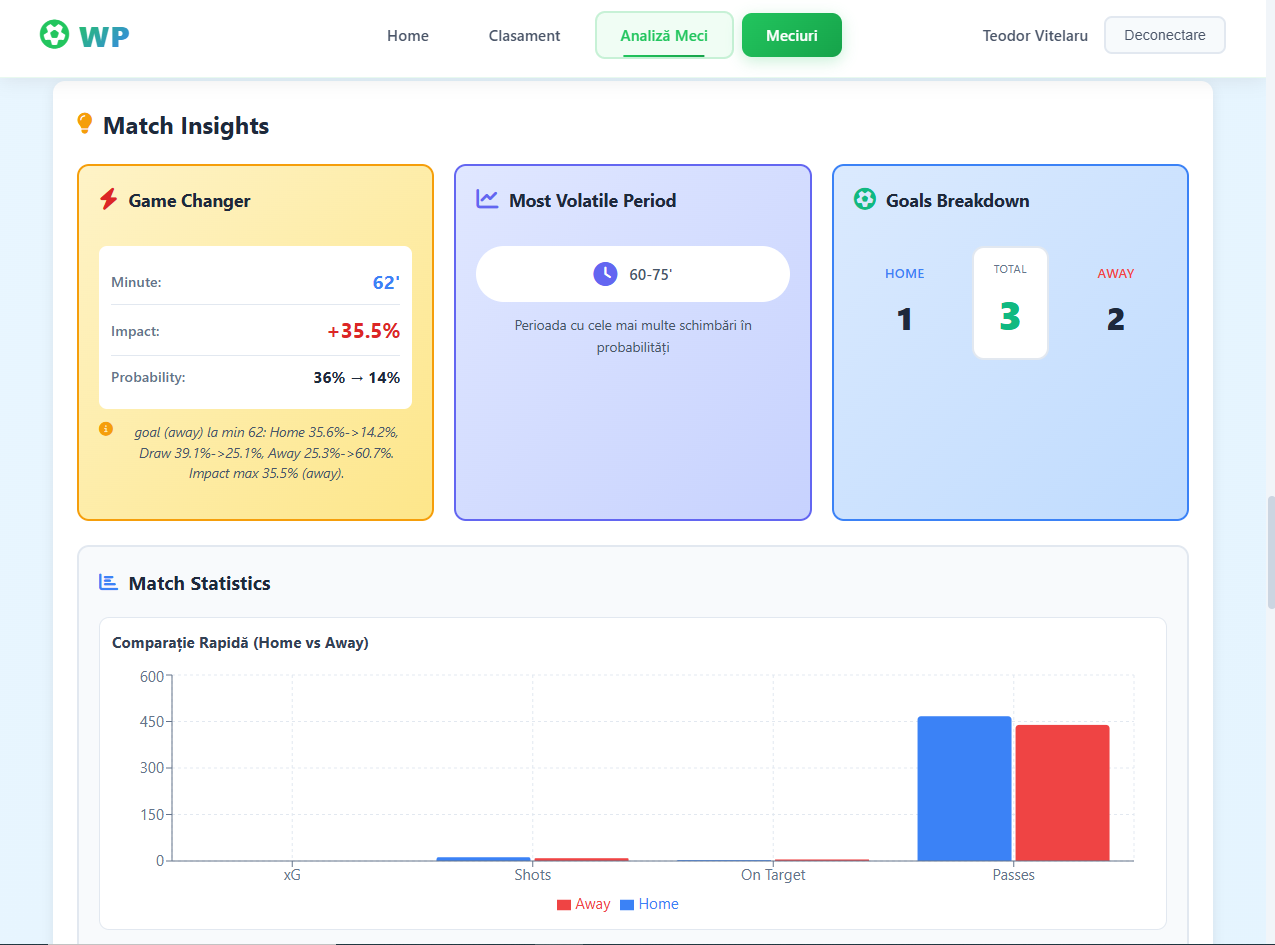
\includegraphics[width=0.85\textwidth]{figures/descriere3.png}
    \caption{Secțiunea \textit{Match Insights} pentru meciul CFR 1907 Cluj
    contra Farul Constanța: \textit{Game Changer} în minutul 62 cu impact
    +35.5\% în favoarea Farului Constanța (probabilitate gazdă de la 35.6\%
    la 14.2\%), perioada cea mai volatilă 60-75' și comparația statisticilor
    brute între cele două echipe.}
    \label{fig:match_insights}
\end{figure}

A patra componentă, \textit{Match Timeline - Dominance}, împarte meciul în
intervale de 15 minute și afișează pentru fiecare interval distribuția
probabilităților, indicând echipa dominantă în acea perioadă. Aceasta
permite identificarea fazelor în care controlul s-a schimbat, independent de
momentul golurilor (Figura~\ref{fig:timeline_dominance}).

\begin{figure}[H]
    \centering
    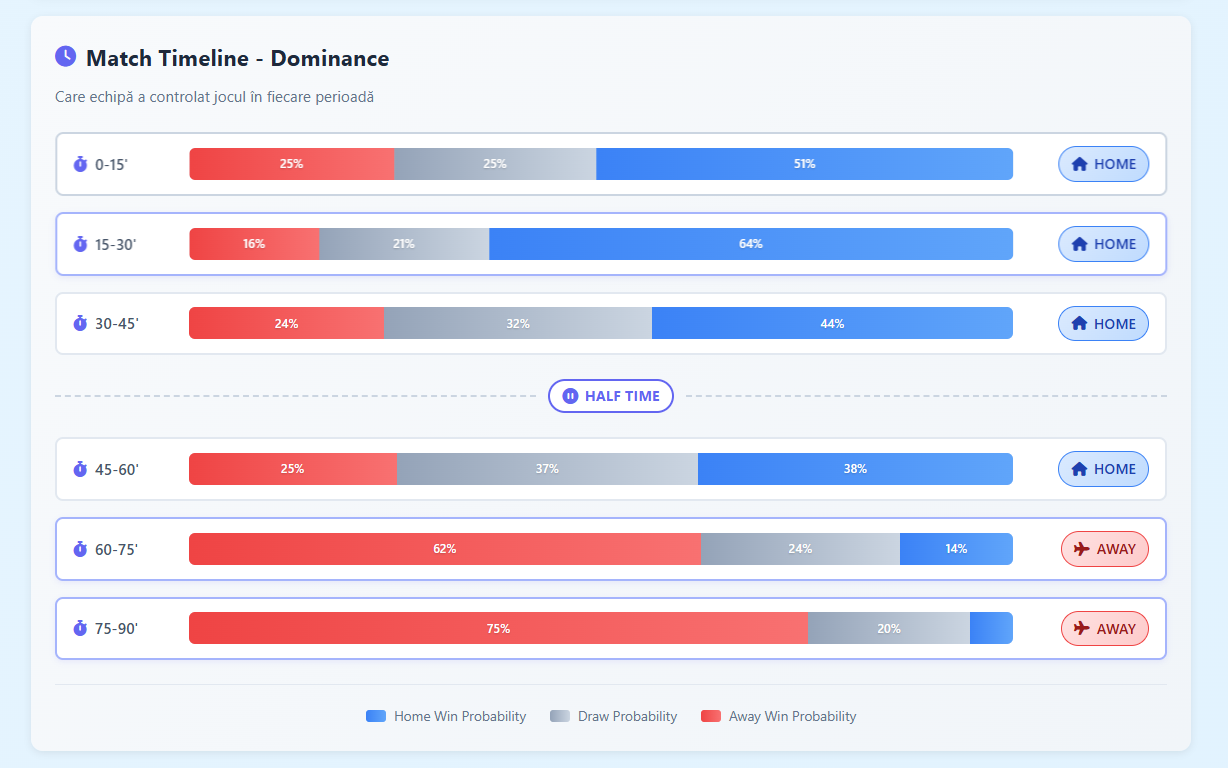
\includegraphics[width=0.85\textwidth]{figures/descriere4.png}
    \caption{\textit{Match Timeline - Dominance} pentru meciul CFR 1907 Cluj
    contra Farul Constanța: CFR Cluj a dominat primele 60 de minute
    (probabilitate de câștig 44-64\% în intervalele 0-45'), în timp ce Farul
    Constanța a preluat controlul decisiv în intervalul 60-75' (62\% victorie
    oaspeți) și l-a menținut până la final (75\% în intervalul 75-90').}
    \label{fig:timeline_dominance}
\end{figure}

\textbf{Pasul 5, vizualizarea istoricului.} Predicția generată este salvată
automat și poate fi regăsită în pagina \textit{Predicții}
(Figura~\ref{fig:manual_predictions}), unde toate predicțiile sunt
organizate pe echipe. Utilizatorul poate astfel urmări evoluția
probabilistică a echipelor de-a lungul sezonului.

\begin{figure}[H]
    \centering
    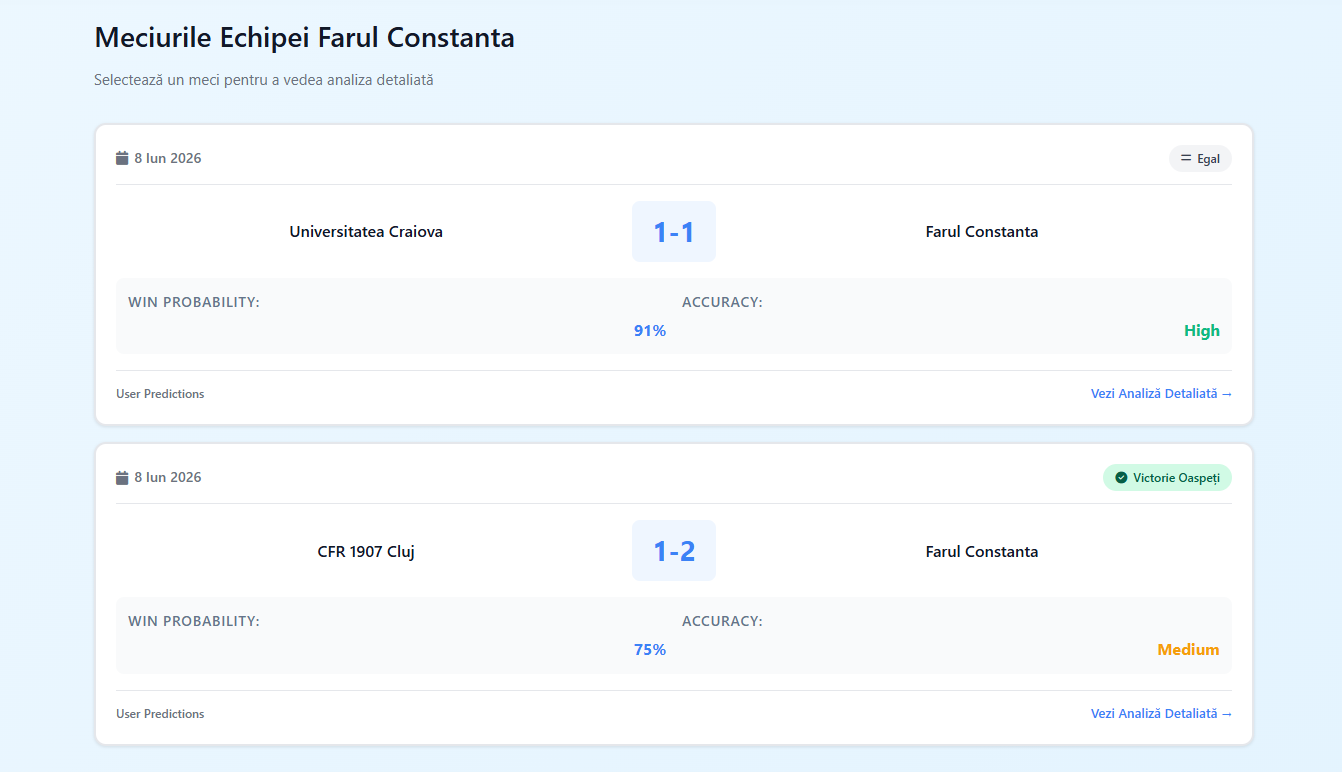
\includegraphics[width=0.82\textwidth]{figures/screenshot_predictions.png}
    \caption{Pagina de predicții salvate, organizate pe echipe.}
    \label{fig:manual_predictions}
\end{figure}
